\begin{block}{Motivation}
 
 \begin{figure}[H]
\centering
\newcommand{\robot}[4]{
\begin{scope}[shift={(#1,#2)}, scale=#3]
\tikzset{
  point/.style={circle, fill=black, inner sep=1.8pt}
}

% Head
\draw[rounded corners=3pt, fill=gray!20] (-1,1) rectangle (1,3);

% Eyes (use color parameter)
\fill[#4] (-0.5,2.2) circle (0.15);
\fill[#4] (0.5,2.2) circle (0.15);

% Mouth
\draw[line width=0.8pt] (-0.4,1.6) -- (0.4,1.6);

% Antenna
\draw[line width=0.8pt] (0,3) -- (0,3.6);
\fill[#4] (0,3.6) circle (0.15);

% Body
\draw[rounded corners=5pt, fill=gray!10] (-1.5,-1) rectangle (1.5,1);

% Buttons (also colored)
\fill[#4] (0,0.3) circle (0.15);
\fill[#4] (0,-0.2) circle (0.15);
\fill[#4] (0,-0.7) circle (0.15);

% Arms
\draw[line width=0.8pt] (-1.5,0.5) -- (-2.2,0.5);
\draw[line width=0.8pt] (1.5,0.5) -- (2.2,0.5);

% Hands
\fill[#4] (-2.2,0.5) circle (0.12);
\fill[#4] (2.2,0.5) circle (0.12);

% Legs
\draw[line width=0.8pt] (-0.6,-1) -- (-0.6,-2);
\draw[line width=0.8pt] (0.6,-1) -- (0.6,-2);

% Feet
\draw[line width=1.5pt] (-0.9,-2) -- (-0.3,-2);
\draw[line width=1.5pt] (0.3,-2) -- (0.9,-2);

\end{scope}
}


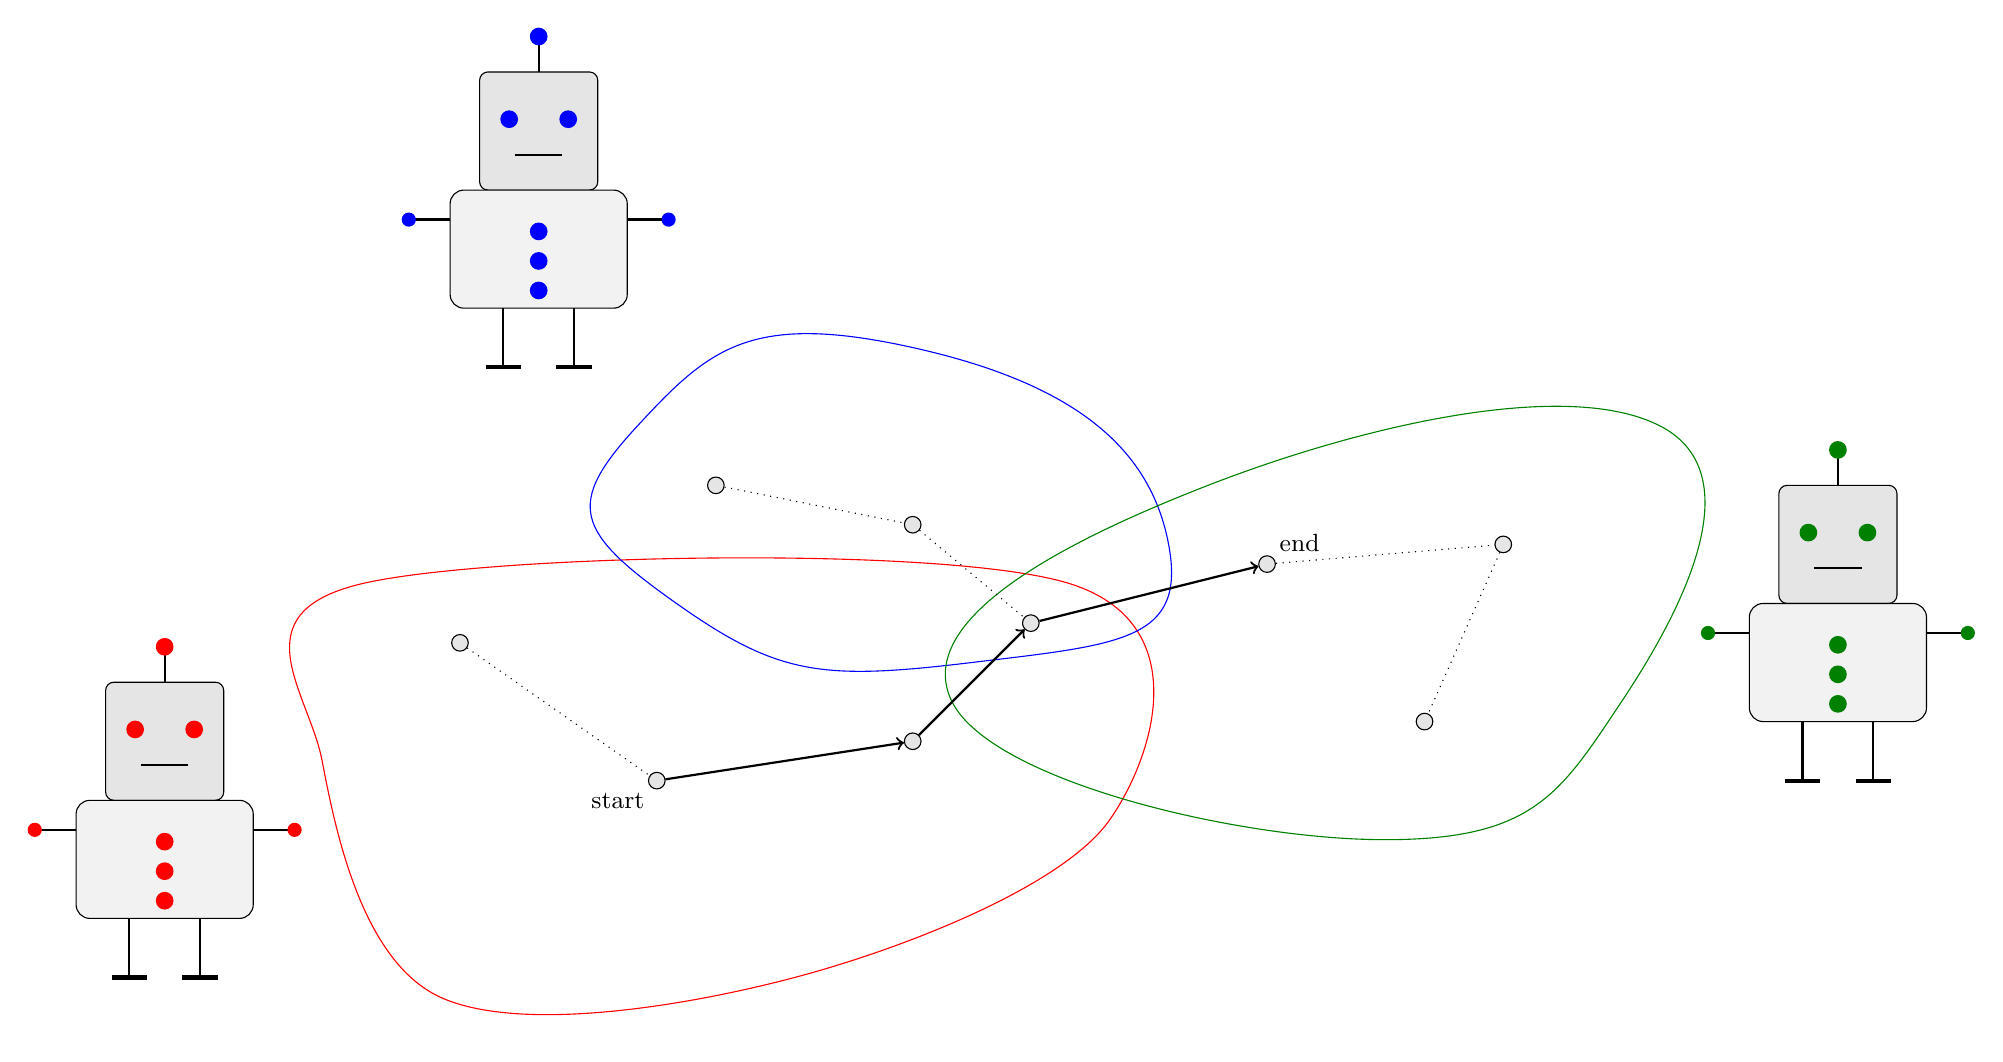
\begin{tikzpicture}[
    scale=2.5,  
    vertex/.style={
        circle,
        draw,
        fill=black!10,
        minimum size=6pt,
        inner sep=0pt
    }
]

% Subgraph boundaries

\robot{-3}{-1}{0.3}{red}
\draw[red] plot [smooth cycle, tension=0.6] coordinates
{(-2.2,-0.5) (-2,0.4) (1.6,0.4)  (1.8,-0.8) (0.2,-1.6) (-1.6,-1.7)};

\robot{-1.1}{2.1}{0.3}{blue}
\draw[blue]  plot [smooth cycle, tension=1.1] coordinates
{(-0.6,1.2) (0.8,1.6) (2.1,0.6) (1.1,0) (-0.4,0.3)};

\robot{5.5}{0}{0.3}{green!50!black}
\draw[green!50!black] plot [smooth cycle, tension=0.8] coordinates
{(2.3,0.9) (4.6,1.2) (4.4,-0.2) (3.2,-0.9) (1.0,-0.2)};

% G1 vertices
\node[vertex] (a1) at (-1.5,0.1) {};
\node[vertex] (a2) at (-0.5,-0.6) {};
\node[vertex] (a3) at (0.8,-0.4) {};
\draw[dotted] (a1) -- (a2) -- (a3);

% G2 vertices
\node[vertex] (b1) at (-0.2,0.9) {};
\node[vertex] (b2) at (0.8,0.7) {};
\node[vertex] (b3) at (1.4,0.2) {};
\draw[dotted] (b1) -- (b2) -- (b3);

% G3 vertices
\node[vertex] (c1) at (2.6,0.5) {};
\node[vertex] (c2) at (3.8,0.6) {};
\node[vertex] (c3) at (3.4,-0.3) {};
\draw[dotted] (c1) -- (c2) -- (c3);

% Labels
\node[below left=1pt] at (a2) {\small start};
\node[above right=1pt] at (c1) {\small end};

% Cross connections
\draw[thick, <-] (c1) -- (b3);
\draw[thick, <-] (b3) -- (a3);
\draw[thick, <-] (a3) -- (a2);


\end{tikzpicture}
\caption{Path in Agent Owned Graphs}
\end{figure}

Many real-world systems involve multiple agents coordinating, such as self-driving cars, airports, or distributed servers. Each agent has only partial information, so communication is required to solve the shared task. This begs the question:

\vspace{0.5em}

\begin{center}
\textit{How much communication is fundamentally necessary?}
\end{center}

\end{block}

\begin{block} {Two Party Communication Complexity} 

Communication Complexity studies the minimum number of bits that multiple parties must exchange to compute a function when the input is distributed.

\medskip

Instead of asking: \textit{How fast is the algorithm?}\\
We ask: \textit{How much communication is needed within the algorithm?}


\end{block}

\begin{block}{Two Party Communcation Complexity} 

There are two players, traditionally called \textbf{Alice} and \textbf{Bob}.  
\begin{itemize}
    \item Alice holds input $x$
    \item Bob holds input $y$
\end{itemize}

Neither of them knows the inputs of the other persons, so they must talk back and forth until they know enough to compute some function $f(x,y)$

\begin{figure}[H]
\centering
\begin{tikzpicture}[scale=1.5]

% ---------- Alice ----------
\draw (0,0) circle (0.5);            
\draw (0,-0.5) -- (0,-2);             
\draw (0,-1) -- (-0.8,-1.5);          
\draw (0,-1) -- (0.8,-1.5);          
\draw (0,-2) -- (-0.6,-3);           
\draw (0,-2) -- (0.6,-3);             
\node at (0,-3.6) {$Alice: x$};


% ---------- Bob ----------
\draw (12,0) circle (0.5);              
\draw (12,-0.5) -- (12,-2);              
\draw (12,-1) -- (11.2,-1.5);            
\draw (12,-1) -- (12.8,-1.5);            
\draw (12,-2) -- (11.4,-3);              
\draw (12,-2) -- (12.6,-3);              
\node at (12,-3.6) {$Bob: y$};

% ---------- Speech bubble from Alice ----------
\draw[rounded corners=10pt] 
(2,0.5) rectangle (8,2);

\node at (5,1.2) {\small ``My first bit is 1''};
\draw (1,0.5) -- (2,1);
\draw (1,0.5) -- (2,1.5);



% ---------- Speech bubble from Bob ----------
\draw[rounded corners=10pt] 
(3.5,-2) rectangle (9.5,-0.5);
\node at (6.5,-1.3) {\small ``My third bit is 0''};
\draw (9.5,-1) -- (11,-0.5); 
\draw (9.5,-1.5) -- (11,-0.5);  


\end{tikzpicture}
\caption{Alice and Bob exchanging messages.}
\end{figure}
\end{block}

\begin{block} {Maximally Hard} 

In the worst case, Alice just send all $n$ bits. This is called \textbf{maximally hard}.

\begin{figure}[H]
\centering
\begin{tikzpicture}[scale=1.5]

% ---------- Alice ----------
\draw (0,0) circle (0.5);            
\draw (0,-0.5) -- (0,-2);             
\draw (0,-1) -- (-0.8,-1.5);          
\draw (0,-1) -- (0.8,-1.5);          
\draw (0,-2) -- (-0.6,-3);           
\draw (0,-2) -- (0.6,-3);             
\node at (0,-3.6) {$Alice: x$};


% ---------- Bob ----------
\draw (12,0) circle (0.5);              
\draw (12,-0.5) -- (12,-2);              
\draw (12,-1) -- (11.2,-1.5);            
\draw (12,-1) -- (12.8,-1.5);            
\draw (12,-2) -- (11.4,-3);              
\draw (12,-2) -- (12.6,-3);              
\node at (12,-3.6) {$Bob: y$};

% ---------- Speech bubble from Alice ----------
\draw[rounded corners=10pt] 
(2,0.5) rectangle (8,2);

\node at (5,1.2) {\small ``I give up, my number is 5''};
\draw (1,0.5) -- (2,1);
\draw (1,0.5) -- (2,1.5);



% ---------- Speech bubble from Bob ----------
\draw[rounded corners=10pt] 
(3.5,-2) rectangle (9.5,-0.5);
\node at (6.5,-1.3) {\small ``Ok now I know everything''};
\draw (9.5,-1) -- (11,-0.5); 
\draw (9.5,-1.5) -- (11,-0.5);  


\end{tikzpicture}
\caption{Alice and Bob in Maximally Hard case}
\end{figure}

\end{block}






